\documentclass[
    linespread = 1.25
]{ctexart}
\pagestyle{plain}
\ctexset{
    section/format = \Large\bfseries\raggedright,
    section/number = {\chinese{section}、},
    section/aftername = {\enskip},
    abstractname = {\zihao{-2}摘\quad 要}
}
\usepackage[table,xcdraw]{xcolor}
\usepackage[a4paper, lmargin=1in, rmargin=1in, tmargin=1in, bmargin=1in]{geometry}
\usepackage{amsmath}
\usepackage{booktabs}
\usepackage{graphicx}
\graphicspath{ {./fig} }

\usepackage{listings}
\usepackage{color}

\usepackage[sorting=none]{biblatex}
\addbibresource{LLMTuningReport.bib}

\definecolor{dkgreen}{rgb}{0,0.6,0}
\definecolor{gray}{rgb}{0.5,0.5,0.5}
\definecolor{mauve}{rgb}{0.58,0,0.82}

\lstset{
  frame=tb,
  language=Python,
  aboveskip=3mm,
  belowskip=3mm,
  showstringspaces=false,
  columns=flexible,
  basicstyle={\small\ttfamily},
  numbers=left,
  numberstyle=\tiny\color{gray},
  keywordstyle=\color{blue},
  commentstyle=\color{dkgreen},
  stringstyle=\color{mauve},
  breaklines=true,
  breakatwhitespace=true,
  tabsize=2
}
\usepackage{amssymb}
\usepackage[hidelinks]{hyperref}
\usepackage{caption}
\usepackage{subcaption}
\usepackage{siunitx}
\usepackage{algorithm2e}
\SetAlgoInsideSkip{bigskip}
\SetAlgorithmName{算法}{算法}{算法}
\RestyleAlgo{ruled}
\usepackage{multicol}
\usepackage{longtable}
\usepackage{tablefootnote}


\title{\zihao{2}\textbf{大数据创新实践实验报告}\\\zihao{3}\textbf{——多模态大模型LLaVA的微调}}
\author{\zihao{4}曹瀚文 \\\texttt{学号:210810503}
\and \zihao{4}岑畅 \\\texttt{学号:210810501}
\and \zihao{4}丁有罡 \\\texttt{学号:210810518}
\and \zihao{4}符永宣\\\texttt{学号:210810506}
\and \zihao{4}金文韬\\\texttt{学号:210810306}
\and \zihao{4}刘炎培\\\texttt{学号:210810510}
\and \zihao{4}刘梓涛\\\texttt{学号:210810513}
\and \zihao{4}彭珂\\\texttt{学号:210810508}
\and \zihao{4}王子霖\\\texttt{学号:210810522}
\and \zihao{4}文宇祥\\\texttt{学号:210810514}
}
\date{}

\begin{document}

\begin{titlepage}
  \newgeometry{top=1in,bottom=1in,right=0.75in,left=0.75in}
  \maketitle
  \vspace{0.2cm}
  \begin{abstract}
    \zihao{-4}
    \vspace{0.8cm}
    \linespread{1.25}
    本论文主要研究了空气质量、污染物水平及其与时空、气候因素的关系,并基于历史数据预测未来空气质量。论文首先对数据进行了预处理,包括数据描述、数据标准化、异常值及缺失值处理、极值值处理等步骤。接着,采用系统聚类方法对不同城市的污染物水平进行了潜在模式探索,通过均值和不同邻距离的聚类方法分析得出了系统聚类结果,并用因子分析的得分对其进行了解释。

    论文进一步探讨了空气质量与时空、气候因素的相关关系,应用多元线性回归模型和改进的多元线性回归模型,诊断模型结果并分析了气候因素与空气质量之间的相关性。此外,论文介绍并应用了广义线性模型,实现利用时空、气候因素对空气质量进行更加准确的预测。

    最后,论文利用SARIMA模型和GARCH模型,根据历史空气质量数据预测未来一段时间内的空气质量,以南昌市为例进行了实证研究。通过数据导入、探索性期性、参数确定、模型诊断及预测等步骤,详细展示了两种模型的应用过程和预测效果。

    本文不仅揭示了不同城市空气污染物可能存在的潜在模式,同时探究了空气质量与多种因素之间的复杂关系,也为空气质量的预测提供了有效的模型和方法,对城市环境管理、污染控制和空气质量的预报具有重要的参考价值。

    \vspace{1cm}
    \noindent\textbf{关键词:} 系统聚类\hspace{0.22cm} 因子分析\hspace{0.22cm} 多元线性回归\hspace{0.22cm} 广义线性模型\hspace{0.22cm} 时间序列分析
  \end{abstract}
\end{titlepage}

\tableofcontents
\newpage
\section{实验背景}
在当今人工智能和机器学习领域,预训练大规模语言模型(如GPT-4)已经展现出卓越的性能。然而,尽管这些模型在许多任务中表现优异,它们的通用性仍然可能无法满足特定应用场景的需求。因此,为了进一步提升模型在特定领域的效果,参数微调成为了一个关键的研究方向。通过微调,我们可以根据特定的数据集和任务需求对模型进行定制,使其在处理特定类型的输入时表现得更加精准和高效。这种方法不仅可以改善模型的预测能力,还能提升其对领域特定知识的理解和应用能力。为了实现最佳的微调效果,研究者们通常需要细致地调整模型的超参数,探索不同的优化策略,以便找到最适合特定应用场景的配置。

本次参数微调实验旨在通过自动驾驶数据集对LLaVA模型进行微调,以期提升该模型在自动驾驶领域的综合表现。同时,在该过程中我们希望探究微调过程中的关键影响因素,并采用多种方法评估微调效果。

% 本次实验选取的模型是开源的大语言模型LLaVA\cite{liu2023llava},该模型结合了语言模型和视觉模型,能够同时处理文本和图像输入,从而更好地理解和生成多模态信息,如图\ref{fig:LLaVA}所示。LLaVA通过大规模预训练学习到丰富的特征表示,并在特定任务中通过微调进一步优化性能,在自动驾驶、医疗影像分析、智能客服和内容创作等多个领域展现出广泛的应用前景和高效的推理性能。

% 本次实验将采用的是LoRA(Low-Rank Adaptation)参数微调算法\cite{hu2021loralowrankadaptationlarge},它是一种高效的参数微调方法,通过在预训练模型的权重矩阵上添加低秩分解来减少参数数量,如图\ref{fig:LoRA}所示。这种方法不仅显著降低了微调过程中所需的计算资源和存储空间,还能在保持模型性能的同时,快速适应新的任务和数据。LoRA通过只微调一小部分参数,使得大规模预训练模型的应用更加灵活和经济。

\begin{figure}[htbp]
  \centering
  \begin{minipage}[b]{0.6\textwidth}
    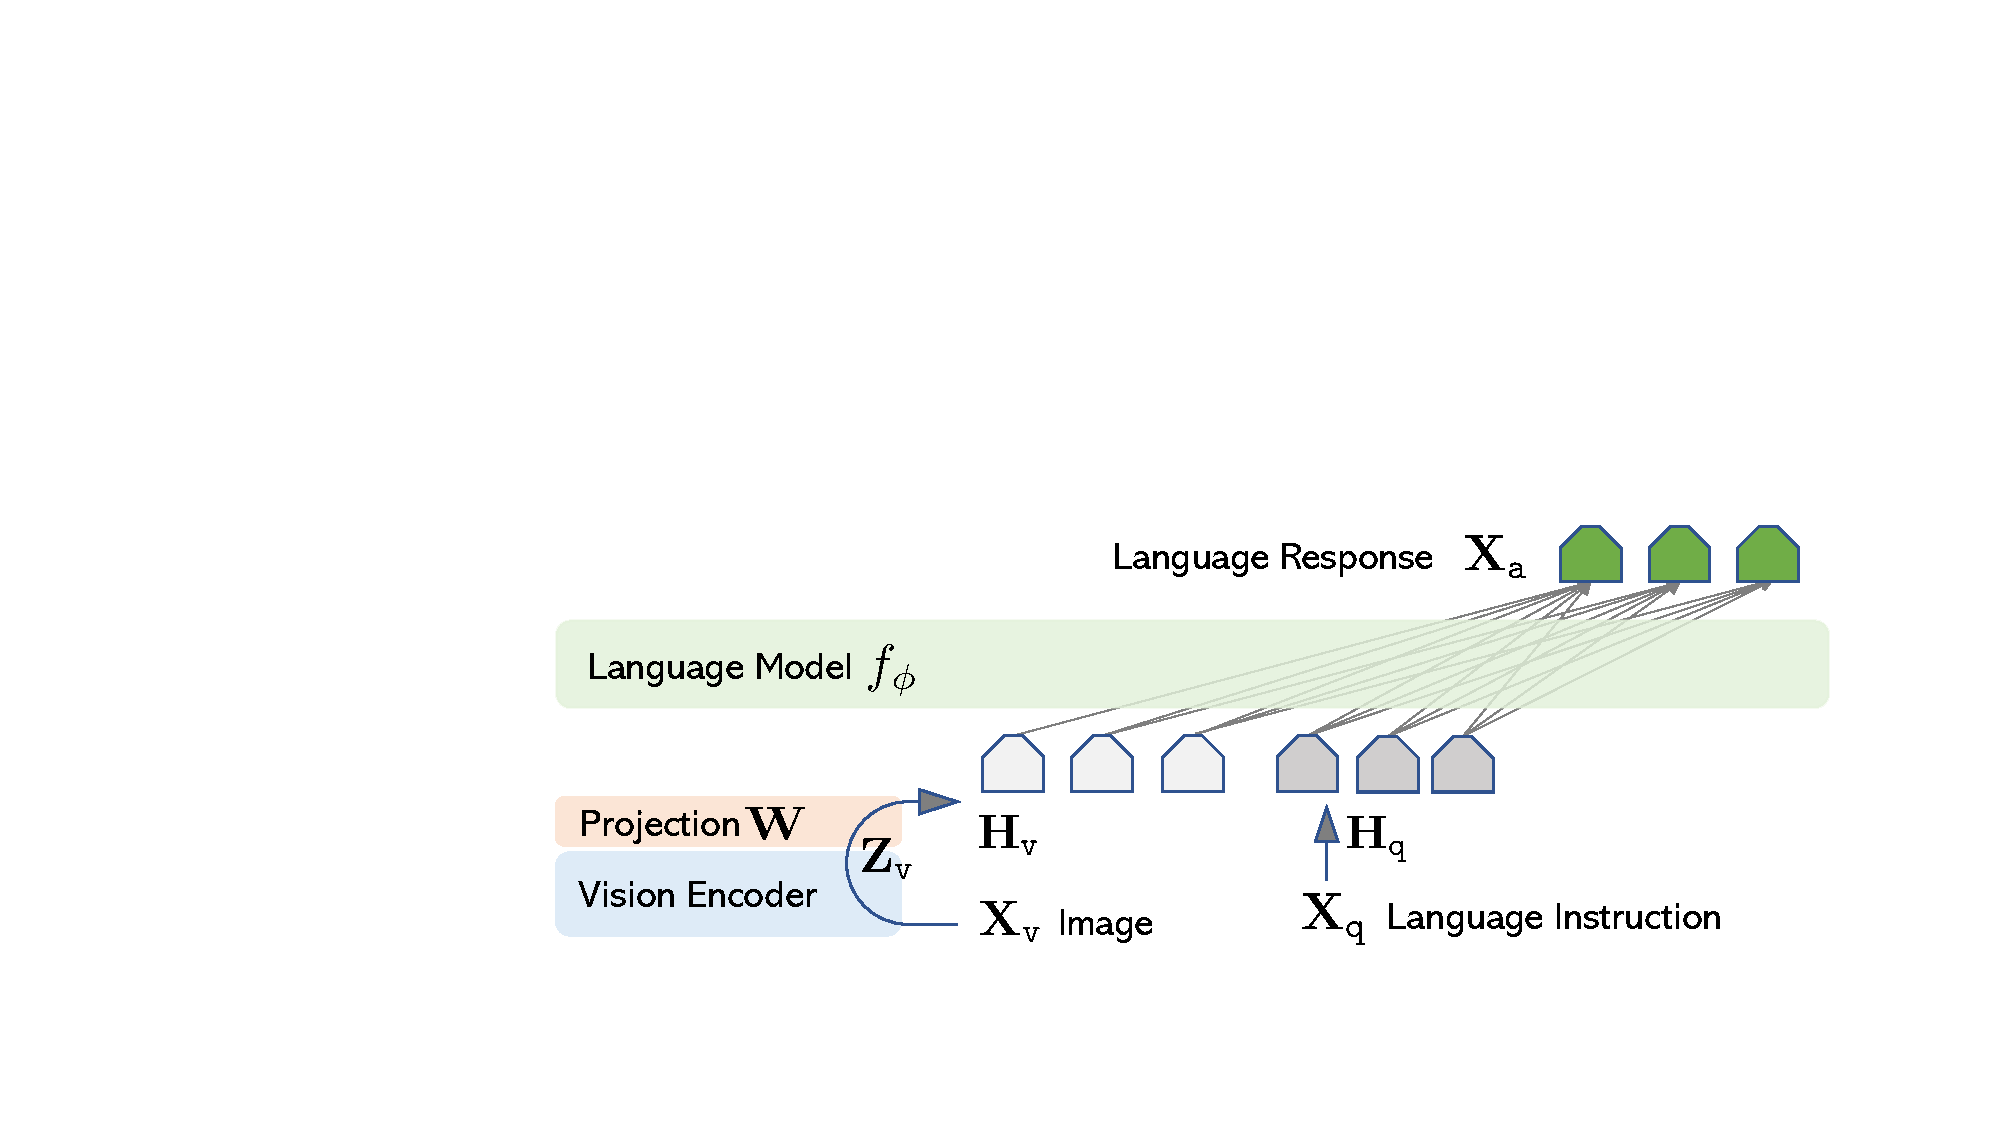
\includegraphics[width=\textwidth]{illu_llava.pdf}
    \caption{LLaVA模型架构}
    \label{fig:LLaVA}
  \end{minipage}
  \hfill
  \begin{minipage}[b]{0.25\textwidth}
    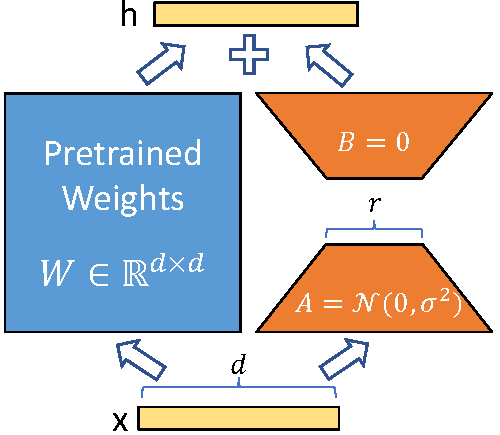
\includegraphics[width=\textwidth]{illu_lora.pdf}
    \caption{LoRA算法图解}
    \label{fig:LoRA}
  \end{minipage}
\end{figure}

% 本次实验在黎勃老师提供的Linux服务器平台上进行,通过SSH远程连接服务器进行实验。

\section{基于自动驾驶数据集的模型微调}

% \subsection{LoRA参数微调算法简介}

\subsection{使用LoRA算法和自动驾驶数据集对LLaVA模型作指令微调}

\subsection{实现微调模型的图形化界面}

\subsection{结论}

\section{探索影响微调效果的实验因素}

\subsection{探究训练周期对微调效果的影响}

\subsection{探究模型大小对微调效果的影响}

\subsection{结论}

\section{使用CODA-LM数据集进行评估}
\subsection{数据集介绍}
CODA-LM 是一个用于自动驾驶边缘情况的大型视觉语言模型(Large Vision-Language Models)评估基准。这个数据集采用分层数据结构,可以促使LVLMs分析复杂的驾驶场景,并生成高质量的预注释供人工注释者进一步验证和修订。CODA-LM旨在提供一个自动化和量化的评估方法,用于解决自动驾驶系统在处理真实世界的边缘情况时常见的挑战。

如表\ref{CODA-LM dataset}中所示,CODA-LM 是首个采用分层评估框架的大规模多模式自动驾驶道路拐角案例数据集。其中包含了三种任务:一般感知、区域感知和驾驶建议。为了更好地理解CODA-LM数据集的评估指标,我们详细介绍一下这三个任务:

\begin{enumerate}
  \item \textbf{一般感知 (General Perception):}
        这个任务的基础在于全面理解驾驶场景中关键的道路实体,包括它们的外观、位置,以及它们如何影响自我车辆的驾驶行为。这个任务对于评估大型视觉语言模型(LVLMs)在解释复杂交互场景中的熟练程度至关重要,仿佛在镜像自动驾驶中的感知过程。此外,为了全面评估LVLMs在不同环境下的表现,数据集根据时间和天气条件对图像进行分类,包括夜间和白天场景,以及晴朗、多云和雨天的天气条件。

  \item \textbf{区域感知 (Regional Perception):}
        这个任务衡量LVLMs在提供特定边界框时理解边缘案例对象的能力,涉及描述给定边界框内的对象以及解释它们为何会影响自动驾驶行为。建立区域感知基于一个核心认识——精确定位边缘案例对于提高系统在自动驾驶实际应用中的整体稳健性至关重要。这些情景通常包含复杂或不寻常的元素,传统模型可能会忽视或难以正确解释,例如独特的交通标志、行为异常的行人和非典型的道路条件。通过专注于这些案例,可以全面了解模型理解边缘案例对象的能力。

  \item \textbf{驾驶建议 (Driving Suggestions):}
        这个任务旨在评估LVLMs制定驾驶建议的能力,这是可解释自动驾驶的一个关键组成部分。这个任务与自动驾驶的规划过程密切相关,要求模型在正确感知当前驾驶环境的一般和区域方面后,为自我车辆提供最佳的驾驶建议。通过构建驾驶建议任务,可以深入评估LVLMs在制定有效驾驶策略方面的表现。
\end{enumerate}

\begin{table}[h]
  \centering
  % \small
  \caption{Comparison between CODA-LM and existing datasets.}
  \label{CODA-LM dataset}
  \begin{tabular}{@{}lccccc@{}}
    \toprule
    \textbf{Dataset} & \textbf{Multimodal}         & \textbf{Corner}             & \textbf{General Per.} & \textbf{Regional Per.}      & \textbf{Suggestion}         \\
    \midrule
    CODA             & \textcolor{red}{\textbf{X}} & \checkmark                  & \checkmark            & \checkmark                  & \textcolor{red}{\textbf{X}} \\
    StreetHazards    & \textcolor{red}{\textbf{X}} & \checkmark                  & \checkmark            & \checkmark                  & \textcolor{red}{\textbf{X}} \\
    \midrule
    nuScenes-QA      & \checkmark                  & \textcolor{red}{\textbf{X}} &
    \checkmark       & \textcolor{red}{\textbf{X}} & \textcolor{red}{\textbf{X}}                                                                                     \\
    BDD-X            & \checkmark                  & \textcolor{red}{\textbf{X}} & \checkmark            & \textcolor{red}{\textbf{X}} & \textcolor{red}{\textbf{X}} \\
    DRAMA            & \checkmark                  & \textcolor{red}{\textbf{X}} & \checkmark            & \checkmark                  & \checkmark                  \\
    DriveLM          & \checkmark                  & \textcolor{red}{\textbf{X}} & \checkmark            & \checkmark                  & \checkmark                  \\
    \rowcolor[HTML]{DAE8FC}
    \midrule
    CODA-LM          & \checkmark                  & \checkmark                  & \checkmark            & \checkmark                  & \checkmark                  \\
    \bottomrule
  \end{tabular}
\end{table}

此外,CODA-LM 数据集通过结构化的文本和人工检查的过程,确保了注释的质量和一致性,从而提高了自动驾驶系统的解释能力和决策质量。这种系统的构建可以显著推动自动驾驶技术的发展,特别是在解决复杂和非标准驾驶场景时的应用。

\subsection{实验过程}

\subsubsection{数据准备}
首先,我们需要下载和准备CODA-LM 数据集。以下是主要步骤概要:

\begin{enumerate}
  \item \textbf{数据下载:}
        \begin{itemize}
          \item 按照 CODA 官方指南下载图像文件。
          \item 下载 CODA-LM 的注释文件,并在同一根目录下解压。
        \end{itemize}

  \item \textbf{数据划分:} 数据集被划分为训练集、验证集、测试集和小型集,具体信息如下:
        \begin{itemize}
          \item Train集:包含 4884 张图像,来源于 CODA2022 的验证集。
          \item Val集:包含 4384 张图像,来源于 CODA2022 的测试集。
          \item Test集:包含 500 张图像,同样来源于 CODA2022 的测试集。
          \item Mini集:50 张图像,为验证集的一个子集,用于演示。
        \end{itemize}
  \item \textbf{数据组织:} 按照要求组织数据,确保图像和注释文件的对应关系正确。
  \item \textbf{数据格式:}
        注释文件包含三个任务的问答对,数据格式如下:
        \begin{verbatim}
    {
        "general_perception": {
            "vehicles": [...],
            "vulnerable_road_users": [...],
            "traffic signs": [...],
            "traffic lights": [...],
            "traffic cones": [...],
            "barriers": [...],
            "other objects": [...],
            "description and explanation": <str>
        },
        "region_perception": {
            "1": {...},
            "2": {...},
            "3": {...}
        },
        "driving_suggestion": <str>
    }
    \end{verbatim}
\end{enumerate}

\subsubsection{数据使用流程}

在下载好数据后,我们将 CODA-LM 数据集转换为基本视觉问答(VQA)格式。以下是流程概要:

\begin{enumerate}
  \item \textbf{运行转换脚本}
        使用 Python 脚本 \texttt{convert2vqa.py} 转换注释数据。根据需要处理的语言版本,可以选择运行英文或中文版本的命令,这里我们选择英文。

  \item \textbf{基本 VQA 格式:}
        VQA 格式的数据采用简单的字典形式保存,包含 \texttt{question\_id}、\texttt{image}、\texttt{question} 和 \texttt{answer}。这种格式便于处理和解析数据,用于视觉问答模型的训练和评估。


  \item \textbf{区域感知的具体实现:}

        对于区域感知,文中提到了一个简单的实现方法:在图像上绘制红色矩形框,保存在 \texttt{images\_w\_bboxes} 目录中。这种方法可以帮助模型学习如何从特定区域中提取信息。

        \begin{figure}[h] % 创建一个图像环境
          \centering % 图片居中
          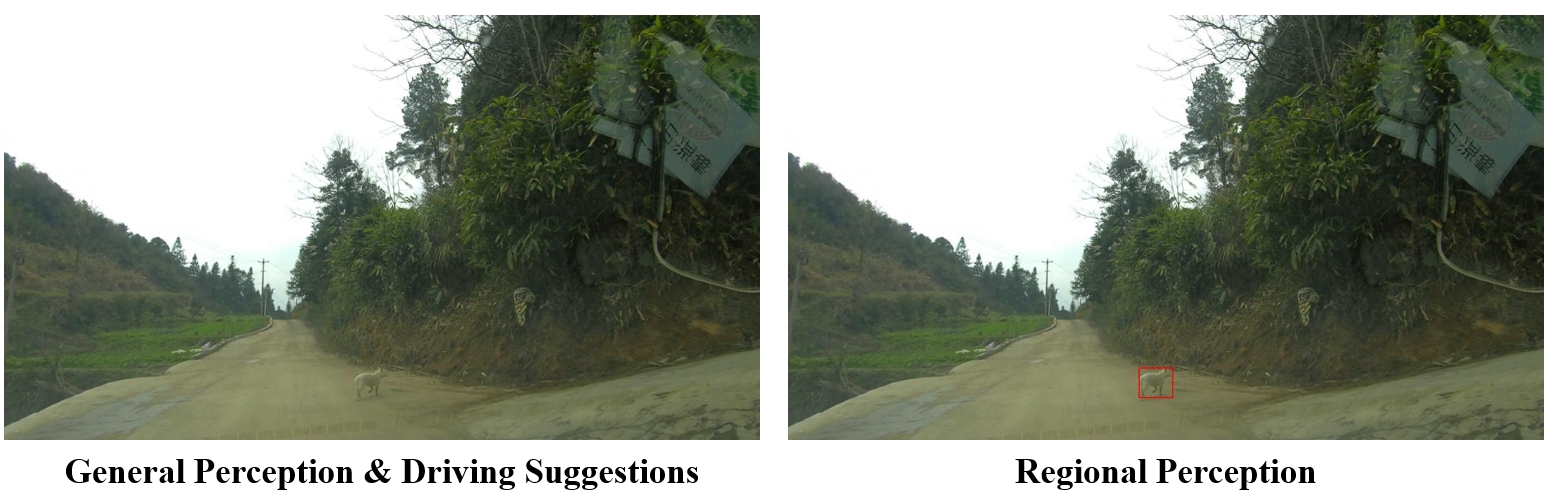
\includegraphics[width=0.5\textwidth]{fig\visual.png} % 插入图片,设置图片宽度为文本宽度的50%
          \caption{区域感知} % 图片标题
          \label{fig:example} % 图片标签,用于引用
        \end{figure}
\end{enumerate}

\subsection{评估结果}

\begin{table}[htbp]
  \centering
  \caption{Comparison of LLaVA model before and after fine-tuning on CODA-LM dataset}
  \small % 调整表格字体大小
  % \renewcommand{\arraystretch}{1.2} % 调整行距
  \begin{tabular}{lcccccccccc}
    \toprule
    \textbf{Method}   & \textbf{General↑}   & \multicolumn{5}{c}{\textbf{Regional Perception↑}} & \textbf{Suggestion↑}                                                                           \\
    \cmidrule(r){3-7}
                      & \textbf{Text-Score} & \textbf{Vehicle}                                  & \textbf{VRU}         & \textbf{Cone} & \textbf{Barrier} & \textbf{Other} & \textbf{Text-Score} \\
    \midrule
    LLaVA1.5-7B       & 19.30               & 46.67                                             & 38.47                & 50.83         & 30.93            & 33.82          & 23.16               \\
    LLaVA1.5-7B+LoRA  & \textbf{20.40}      & 46.03                                             & 36.00                & 45.56         & \textbf{33.57}   & \textbf{40.00} & \textbf{25.20}      \\
    \midrule
    LLaVA1.5-13B      & 24.54               & 53.62                                             & 36.79                & 41.27         & 30.41            & 33.82          & 27.90               \\
    LLaVA1.5-13B+LoRA & \textbf{25.00}      & 53.45                                             & 30.00                & 41.11         & \textbf{40.00}   & \textbf{34.29} & \textbf{29.40}      \\
    \bottomrule
  \end{tabular}
\end{table}

\subsection{结论}

\section{实验结论}

\appendix
\newpage
\section*{参考文献}
\addcontentsline{toc}{section}{参考文献}
\printbibliography[heading=none]
% \noindent
% [1] 乐东明,王文浚,王颖,等. 2020—2022年咸宁市臭氧污染气象特征及成因分析[J].黑龙江环境通报, 2024, 37(05):30-32.

% \noindent
% [2] 李高荣,吴密霞. 多元统计分析[M]. 北京:科学出版社, 2021

% \noindent
% [3] John A. Rice. Mathematical Statistics and Data Analysis[M]. Boston: Cengage Learning, 2006

% \noindent
% [4] 何书元. 应用时间序列分析[M]. 北京:北京大学出版社, 2003

\newpage
\section*{附录:实验日志与心得}
\addcontentsline{toc}{section}{附录:实验日志与心得}

\end{document}

